\section{Referencial do cubesat}

O referencial do cubesat é alinhado geometricamente com o equipamento, dessa forma, ele representa a posição do cubesat em si, 
como pode ser visto na Figura ~\ref{fig:Referencia_do_Cubesat}.

\begin{figure}[H]
	\centering
	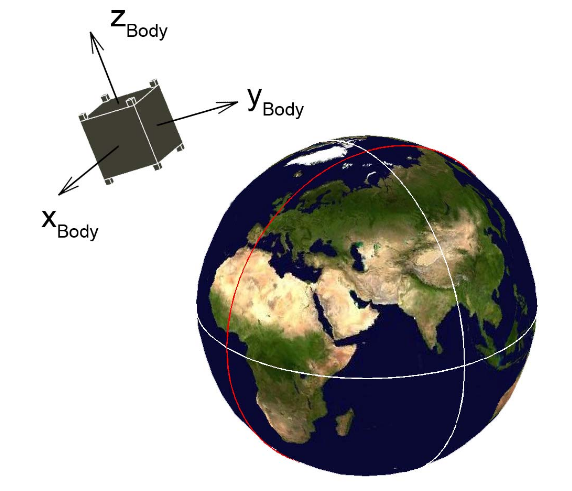
\includegraphics[width=.7\columnwidth]{images/Referencia_do_Cubesat.png}
	\caption{Referência do Cubesat. Fonte: ~\cite[]{Diaz}}
	\label{fig:Referencia_do_Cubesat}
\end{figure}

O referencial da câmera tem os eixos x e y normal ao plano da imagem, a imagem captada pela câmera se encontra a uma distância unitária do cubesat no eixo Z, o motivo de se utilizar uma distância unitária e demais informações sobre o frame de câmera, 
serão tratados no capítulo de projeções em perspectiva. Neste trabalho é considerado que o referencial do cubesat é o mesmo da câmera, como é visto na Figura ~\ref{fig:Camera_Frame}.

\begin{figure}[H]
	\centering
	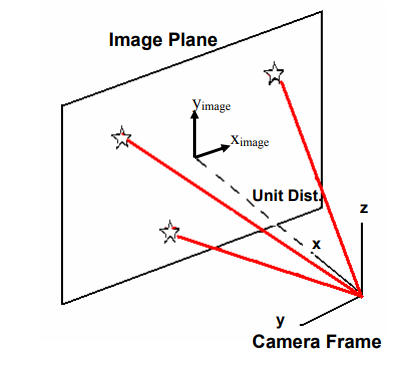
\includegraphics[width=.7\columnwidth]{images/Camera_Frame.png}
	\caption{Camera Frame. Fonte: ~\cite[]{Diaz}}
	\label{fig:Camera_Frame}
\end{figure}